\subsection{Safety Assessment Process}
\label{subsec:process}

ARP4754A, the Guidelines for Development of Civil Aircraft and Systems~\cite{SAE:ARP4754A}, has been recognized by the Federal Aviation Administration (FAA) as an ``acceptable method for establishing a development assurance process''~\cite{AC:20-174}. It provides guidance on applying development assurance at each hierarchical level throughout the development life cycle of highly-integrated/complex aircraft systems.

%Figure~\ref{fig:arp4754a_process} from [ref. ARP4754A] demonstrates the ARP4754A process flow.

The safety assessment process is a starting point at each hierarchical level of the development life cycle, and is tightly coupled with the system development and verification processes. It is used to show compliance with certification requirements, and for meeting a company's internal safety standards~\cite{SAE:ARP4754A}. ARP4761, the Guidelines and Methods for Conducting Safety Assessment Process on Civil Airborne Systems and Equipment~\cite{SAE:ARP4761},  identifies a systematic means to show compliance. The guidelines presented in ARP4761 include industry accepted safety assessment processes (Functional Hazard Assessment (FHA), Preliminary System Safety Assessment (PSSA), and System Safety Assessment (SSA)), and safety analysis methods to conduct the safety assessment, 
such as Fault Tree Analysis (FTA), Failure Modes and Effect Analysis (FMEA), and Common Cause Analysis (CCA).

A prerequisite of performing the safety assessment of a system design is to understand how the system is intended to work, primarily focusing on the integrity of the outputs and the availability of the system. The safety engineers then use the acquired understanding to conduct safety analysis, construct the safety analysis artifacts, and compare the analysis results with established safety objectives and safety-related requirements. 

In practice, prior to performing the safety assessment of a system, the safety engineers are often equipped with the domain knowledge about the system, but do not necessarily have detailed knowledge of the current system is implemented. Acquiring the required knowledge about the behavior and implementation of each software function in a system can be very time-consuming. 

For example, in a recent project it took one of our safety engineers two days to understand how the software in a Stall Warning System was intended to work. The primary task includes connecting the signal and function flows to relate the input and output signals from end-to-end and understanding the causal effect between them. This is at least as much time as was required to contruct the safety analysis artifacts and perform the safety analysis itself. In another instance, it took a safety engineer several months to finalize the PSSA document for a Horizontal Stabilizer Control System, because of two major design revisions requiring multiple rounds of reviews with system, hardware, and software engineers to establish complete understanding of the implemenation details.

Industry practitioners have come to realize the benefits and importance of
using models to assist the safety assessment process (either by augmenting the existing system design model, or by building a separate safety model), and a revision of the ARP4761 to include {\em model based safety analysis} is under way.
Capturing failure modes in models and generating safety analysis artifacts directly from models could greatly improve communication and synchronization between system designer and safety engineers, and provide the ability to more accurately analyze complex systems. 

We believe that using a single unified model to conduct both system development and safety analysis can help reduce the gap in comprehending the system behavior and transferring the knowledge between the system designers and the safety analysts. It maintains a living model that captures the current state of the system design as it moves through the system development lifecycle.
%Figure~\ref{fig:arp4754a_process}.
It also allows all participants of the ARP4754A process to be able to communicate and review the system design using a ``single source of truth.''

A model that supports both system design and safety analysis must describe both the system design information (e.g., system architecture, functional behavior) and safety-relevant information (e.g., failure modes, failure rates).  It must do this in a way that keeps the two types of information distinguishable, yet allows them to interact with each other.

\begin{figure}[t!]
	\vspace{-0.19in}
	\centering
	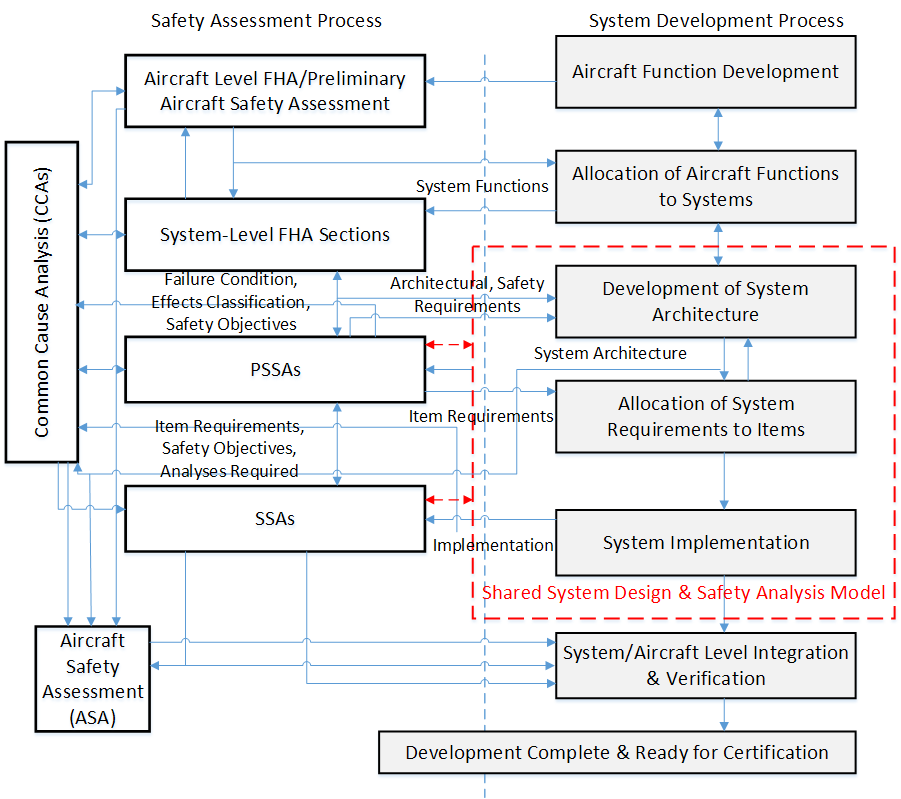
\includegraphics[trim=0 9 0 5,clip,width=0.85\textwidth]{images/Safety_Assessment_Process.png}
	%\vspace{0.4in}
	\caption{Using the Shared System/Safety Model in the ARP4754A Safety Assessment Process}
	\label{fig:proposed_safety_process}
\end{figure}

Figure~\ref{fig:proposed_safety_process} presents our proposed use of this shared system design and safety analysis model in the context of the ARP4754A Safety Assessment Process Model (Figure 7 of ARP4754A). The shared model is one of the system development artifacts from the ``Development of System Architecture'' and ``Allocation of System Requirements to Item'' activities in the System Development Process, which interacts with the PSSAs and SSAs activities in the Safety Assessment Process. The shared model can serve as an interface to capture the information from the system design and implementation that is relevant for the safety analysis.

\begin{figure}[t!]
	\vspace{-0.19in}
	\centering
	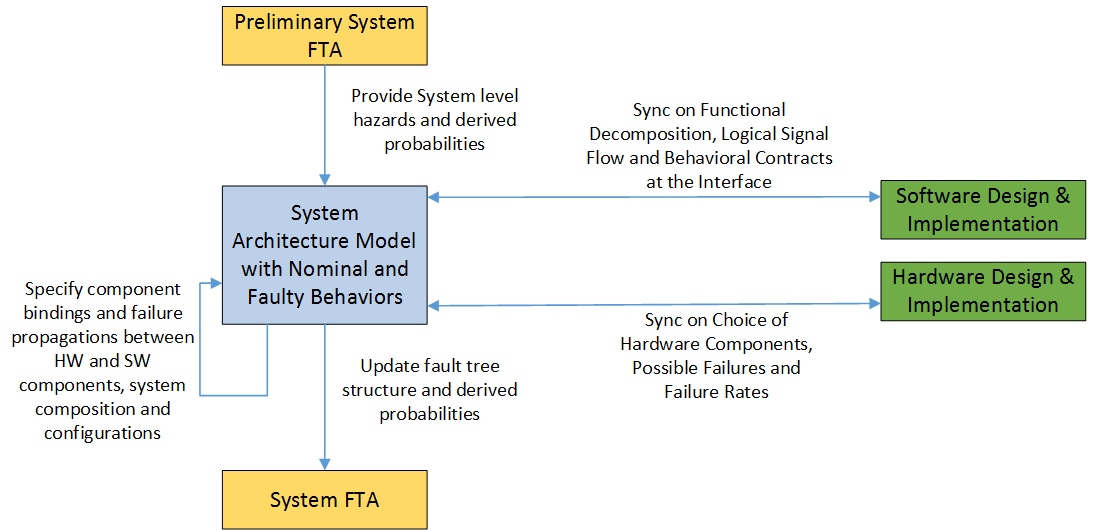
\includegraphics[width=0.9\textwidth]{images/FTA_MBD_Workflow.png}
	%\vspace{-0.19in}
	\caption{Example Interactions between the Shared System/Safety Model and the FTAs}
	\label{fig:interaction_with_FTA}
\end{figure}

Figure~\ref{fig:interaction_with_FTA} shows how the preliminary FTAs and final system FTAs (artifacts from the PSSA and SSA activities in the Safety Assessment Process) can guide and be updated from the shared model.
%\darren{Maybe we need a couple of sentences to explain what's happening in the figure.}
\janet{The shared model is expected to be created and maintained in sync with the software and hardware design and implementation, and guided by the hazard and probability information from the preliminary system FTA. The analysis results from checking the system level properties on the shared model are then used to update the preliminary system FTA. The sync and update process continues iteratively until the system safety property is satisfied with the desired fault tolerance and failure probability achieved. The workload on updating the system FTA from the preliminary system FTA would be greatly reduced.} Next we describe the foundation of the modeling technique in more detail.


